\makeatletter

\mode<presentation>

\usesectionheadtemplate
  {\hfill\insertsectionhead}
  {\hfill\color{fg!50!bg}\insertsectionhead}

\setbeamertemplate{headline}
{%
  \leavevmode%
  \@tempdimb=2.4375ex%
  \ifnum\beamer@subsectionmax<\beamer@sectionmax%
    \multiply\@tempdimb by\beamer@sectionmax%
  \else%
    \multiply\@tempdimb by\beamer@subsectionmax%
  \fi%
  \ifdim\@tempdimb>0pt%
    \advance\@tempdimb by 1.825ex%
    \begin{beamercolorbox}[wd=.5\paperwidth,ht=\@tempdimb]{section in 
    head/foot}%
      \vbox 
      to\@tempdimb{\vfil\insertsectionnavigation{.5\paperwidth}\vfil}%
    \end{beamercolorbox}%
    \begin{beamercolorbox}[wd=.5\paperwidth,ht=\@tempdimb]{subsection in 
    head/foot}%
      \vbox 
to\@tempdimb{\vfil\insertsubsectionnavigation{.5\paperwidth}\vfil}%
    \end{beamercolorbox}
  \fi
  %\vspace*{-\headheight}
}

\usebackgroundtemplate{
\hspace{-1em}
\begin{picture}(250,250)
\put(0,0){
\begin{tikzpicture}
\node (img1)  at (0,0) 
{
\includegraphics[width=1.25\textwidth]{backgroundlight}};
\end{tikzpicture}
}
\put(280,0){
\begin{tikzpicture}
\node (img1)  at (0,0) 
{
\includegraphics[width=15em]{npsglobe}};
\end{tikzpicture}
}
\put(0,0){
\begin{tikzpicture}
\node (img1)  at (0,0) 
{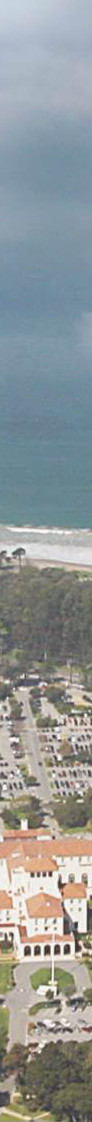
\includegraphics[height=\textheight]{sidepicturethin}};
\end{tikzpicture}
}
\put(0,215) %x=25 for no overlap with sidepicturethin
{
\begin{tikzpicture}[opacity=0.6]
\fill [topbar,blur shadow={shadow blur steps=5}] (30,10) rectangle (5,5);
\end{tikzpicture}
}
\end{picture}
}

\setbeamertemplate{frametitle}{
%\hspace{-0.4cm}
\vskip1em
  \strut\insertframetitle\strut
%\vspace{0.1cm}
%\vbox{\hsize=10cm\bfseries\strut\insertframetitle\strut}
%\vspace{0.1cm}
}

\makeatother